\appendix

\subsection{Motion as second-order systems}%
\label{app:sub:motion_as_second_order_systems}

From natural systems, it can be observed that smooth behavior is the result of second
order differential equations of motion. For example, a pendulum's motion is described by
\begin{equation}
  \ddot{\theta} + \frac{g}{l} sin(\theta) = 0, 
\end{equation}
where $g,l$ as gravity and length are the system's parameter. These parameters will determine
the motion. Due to this observation, it was proposed to describe motion planning as second
order differential equations \cite{Ratliff2020,Ratliff2018}. Specifically, the motion
policy is called \textit{acceleration policy} as the control inputs are accelerations.
In differential geometry,
such secord order differential equations, $\M(\x,\xdot)\xddot + \f(\x,\xdot) = 0$, are
written as tuple $(\M,\f)_{\X}$ and referred to as spectral semi-sprays.

\subsection{Complete list of experiments}%
\label{app:sec:complete_list_of_experiments}

Additional to the experiments shown in the paper, simpler experiments are listed below.


\subsubsection{Experiment 1: Static fabrics vs. MPC}%
\label{app:sub:experiment_1_static_fabrics_vs_mpc}

For the \textbf{point mass}, we randomized the size and location of five obstacles, the initial
configuration and the goal location. Comparisons between both planners for $N=100$ runs
can be found in ~{Fig. \ref{fig:experiment1_pointMass}}. The MPC solver reached an average of
$0.5ms$ of computational time while fabrics took $0.06ms$ to solve the problem in every
time step. The trajectory achieved with fabrics tend to be more conservative as we see in
the increased average clearance in ~{Fig. \ref{subfig:experiment1_pointMass_res}}. 
This finding aligns with the overall increased success rate of fabrics compared to MPC.
The MPC trajectory resulted in collision for 23 cases.
Besides, the time to reach the goal fluctuates significantly for both solvers.

\begin{figure}[h]
  \centering
  \begin{subfigure}{0.7\linewidth}
    \centering
    \includegraphics[height=1.5in]{1_fabric_mpc/pointMass/results}
    \caption{}
    \label{subfig:experiment1_pointMass_res}
  \end{subfigure}%
  \begin{subfigure}{0.3\linewidth}
    \centering
    \includegraphics[height=1.5in]{1_fabric_mpc/pointMass/success}
    \caption{}
    \label{subfig:experiment1_pointMass_success}
  \end{subfigure}
  \caption{Point Mass}%
  \label{fig:experiment1_pointMass}
\end{figure}

Next, a serie of similar experiments was conducted for a \textbf{planar robot} with $n=5$
revolute joints. Collision-free goal locations consisted of randomized end-effector
locations in the plane. The initial configuration was fixed across all runs to $\q_0 =
[0.5\pi, 0, -0.5\pi, 0, 0]^T$. Five randomized obstacles were placed in the workspace.
Comparisons between both planners for $N=100$ runs can be found in ~{Fig.
\ref{fig:experiment1_planarArm}}. The MPC solver reached an average computation time of
$15ms$ while fabrics took around $0.15ms$ to solve the planning problem. Despite tuning,
the time to reach the goal was on average twice as long for fabrics compared to MPC. 
For the planar arm, trajectories obtained with fabrics are more conservative when it comes
to obstacle avoidance and self-collision avoidance. Out of the 100 trajectories obtained
with MPC, 33 were in collision, see ~{Fig. \ref{subfig:experiment1_planarArm_success}}.

\begin{figure}[h]
  \centering
  \begin{subfigure}{0.7\linewidth}
    \centering
    \includegraphics[height=1.5in]{1_fabric_mpc/planarArm/results}
    \caption{}
    \label{subfig:experiment1_planarArm_res}
  \end{subfigure}%
  \begin{subfigure}{0.3\linewidth}
    \centering
    \includegraphics[height=1.5in]{1_fabric_mpc/planarArm/success}
    \caption{}
    \label{subfig:experiment1_planarArm_success}
  \end{subfigure}
  \caption{Planar arm}%
  \label{fig:experiment1_planarArm}
\end{figure}

\begin{figure}[h]
  \centering
  \begin{subfigure}{0.7\linewidth}
    \centering
    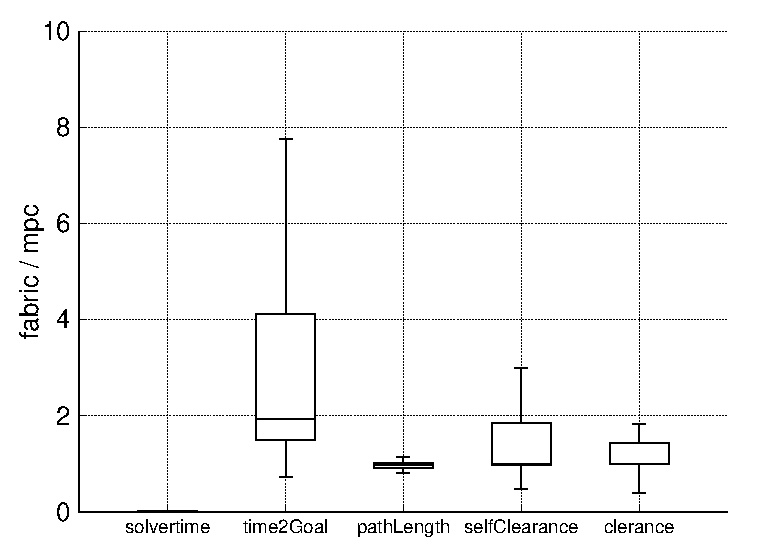
\includegraphics[height=1.5in]{1_fabric_mpc/planarArm/results_long}
    \caption{}
    \label{subfig:experiment1_planarArm_res}
  \end{subfigure}%
  \begin{subfigure}{0.3\linewidth}
    \centering
    \includegraphics[height=1.5in]{1_fabric_mpc/planarArm/success}
    \caption{}
    \label{subfig:experiment1_planarArm_success}
  \end{subfigure}
  \caption{ALTERNATIVE: Planar arm}%
  \label{fig:experiment1_planarArm}
\end{figure}



\subsubsection{Experiment 2: Static fabrics vs. Dynamic fabrics}%
\label{app:sub:experiment_2_static_fabrics_vs_dynamic_fabrics}

We run $N=20$ for an analytic trajectory for the \textbf{pointMass}. The trajectory
\[
  \xt = [-4\sin(0.2t), 4\cos(0.2t)]^T
\]
remained unchanged across all runs. Five obstacles were placed at random inside the
robot's workspace. The initial state was kept unchanged at $\vec{q}_0 = [0.5, 4.5]^T$.
An example of the trajectory can be found in \ref{subfig:experiment2_pointMass_example}.
From the results summarized in \ref{subfig:experiment2_pointMass_res}, we can see that
dynamic fabrics can follow the trajectory more closely (see integratedError), while
solvertime and clearence remain similar.

\begin{figure}[h]
  \centering
  \begin{subfigure}{0.5\linewidth}
    \centering
    \includegraphics[height=1.4in]{2_static_dynamic/pointMass/results}
    \caption{}
    \label{subfig:experiment2_pointMass_res}
  \end{subfigure}%
  \begin{subfigure}{0.5\linewidth}
    \centering
    \includegraphics[width=1.4in]{2_static_dynamic/pointMass/example}
    \caption{}
    \label{subfig:experiment2_pointMass_example}
  \end{subfigure}
  \caption{Experiment2 : Point Mass}%
  \label{fig:experiment2_pointMass}
\end{figure}

Trajectory following for the \textbf{planarArm} with $n=5$ joints
was evaluated with the analytic trajectory
\[
  \xt = [-3.5\cos(0.1t), -3.5\sin(0.1t)].
\]
Across $N=100$ experiments, five obstcalse were placed at random in the robot's workspace.
The initial configuration was kept unchanged at 
\[
  \q_0 = [0.5\pi, 0, -0.5\pi, 0, -0.5\pi]^T.
\]
An example trajectory is visualized in Fig. \ref{subfig:experiment2_planarArm_example}.
Results in terms of integratedError, clerance and solverTime show the same trend as for
the \textbf{pointMass}, see Fig. \ref{subfig:experiment2_planarArm_res}. 

\begin{figure}[h]
  \centering
  \begin{subfigure}{0.5\linewidth}
    \centering
    \includegraphics[height=1.4in]{2_static_dynamic/planarArm/results}
    \caption{}
    \label{subfig:experiment2_planarArm_res}
  \end{subfigure}%
  \begin{subfigure}{0.5\linewidth}
    \centering
    \includegraphics[height=1.4in]{2_static_dynamic/planarArm/example}
    \caption{}
    \label{subfig:experiment2_planarArm_example}
  \end{subfigure}
  \caption{Experiment2 : Planar arm}%
  \label{fig:experiment2_planarArm}
\end{figure}

\subsubsection{Experiment 3: Moving Obstacles}%
\label{app:sub:experiment_3_moving_obstacles}

We evaluated the performance with the \textbf{pointMass} in simulation. In the presented
example the initial configuration \[\q_0 = [0.5, 4.5]^T\] and the obstacle following the
trajectory \[\xt_{\textrm{obst}} = [0.0, -2.5\cos(t)]^T\] remained unchanged while the
goal was randomized in the workspace. The results show that dynamic fabrics are able to
trade path-length and time-to-goal for clearance to the obstacle (Fig.
\ref{subfig:experiment3_pointMass_static_dynamic_res}). This results in an
overall safer motion (Fig. \ref{subfig:experiment3_pointMass_static_dynamic_success}).

\begin{figure}[h]
  \centering
  \begin{subfigure}{0.7\linewidth}
    \centering
    \includegraphics[height=1.5in]{3_moving_obstacles/pointMass/static_dynamic/results}
    \caption{}
    \label{subfig:experiment3_pointMass_static_dynamic_res}
  \end{subfigure}%
  \begin{subfigure}{0.3\linewidth}
    \centering
    \includegraphics[height=1.5in]{3_moving_obstacles/pointMass/static_dynamic/success}
    \caption{}
    \label{subfig:experiment3_pointMass_static_dynamic_success}
  \end{subfigure}
  \caption{Experiment3 : Point Mass, static vs dynamic fabric}%
  \label{fig:experiment3_pointMass}
\end{figure}

\MS{WIP: MPC performs too poorly...}
\begin{figure}[h]
  \centering
  \begin{subfigure}{0.7\linewidth}
    \centering
    \includegraphics[height=1.5in]{3_moving_obstacles/pointMass/dynamic_mpc005/results}
    \caption{}
    \label{subfig:experiment3_pointMass_static_dynamic_res}
  \end{subfigure}%
  \begin{subfigure}{0.3\linewidth}
    \centering
    \includegraphics[height=1.5in]{3_moving_obstacles/pointMass/dynamic_mpc005/success}
    \caption{}
    \label{subfig:experiment3_pointMass_static_dynamic_success}
  \end{subfigure}
  \caption{Experiment3 : Point Mass, MPC(dt=0.05) vs dynamic fabric}%
  \label{fig:experiment3_pointMass}
\end{figure}

We evaluated the performance with the \textbf{planarArm} in simulation. In the presented
example the initial configuration \[\q_0 = [1.0, -0.2]^T\] and the two obstacles following
the trajectories
\begin{align*}
  \xt_{\textrm{obst1}} &= [-1.5, -2.0 + 0.3t]^T \\
  \xt_{\textrm{obst2}} &= [1.5, -2.0 + 0.3t]^T \\
\end{align*}
remained unchanged while the goal was randomized in the workspace. The results for this
robot confirm the findings for the pointMass. Generally, dynamic fabrics are able to keep
a greater distance to moving obstacles while reaching the goal in slightly longer time
(Fig. \ref{fig:experiment3_planarArm}).

\begin{figure}[h]
  \centering
  \begin{subfigure}{0.7\linewidth}
    \centering
    \includegraphics[height=1.5in]{3_moving_obstacles/planarArm/results}
    \caption{}
    \label{subfig:experiment3_planarArm_static_dynamic_res}
  \end{subfigure}%
  \begin{subfigure}{0.3\linewidth}
    \centering
    \includegraphics[height=1.5in]{3_moving_obstacles/planarArm/success}
    \caption{}
    \label{subfig:experiment3_planarArm_static_dynamic_success}
  \end{subfigure}
  \caption{Experiment3 : Planar Arm, static vs dynamic fabric}%
  \label{fig:experiment3_planarArm}
\end{figure}
